%!TEX root = widefieldscan.tex
\svnidlong
{$HeadURL$}
{$LastChangedDate$}
{$LastChangedRevision$}
{$LastChangedBy$}
\framebox{Author: \svnauthor|Rev: \svnrev|Last change: \svndate}% - URL: \url{\svnkw{HeadURL}}}
\section{Results I}
\label{sec: Results I}
A sequence of 19 protocols with varying quality has been scanned to assess the simulations. \todo{show results from R108C21b--R108C21t} which.


\begin{figure}
	\centering
		%\documentclass{article}
%\usepackage{tikz,pgfplots}
%
%\begin{document}

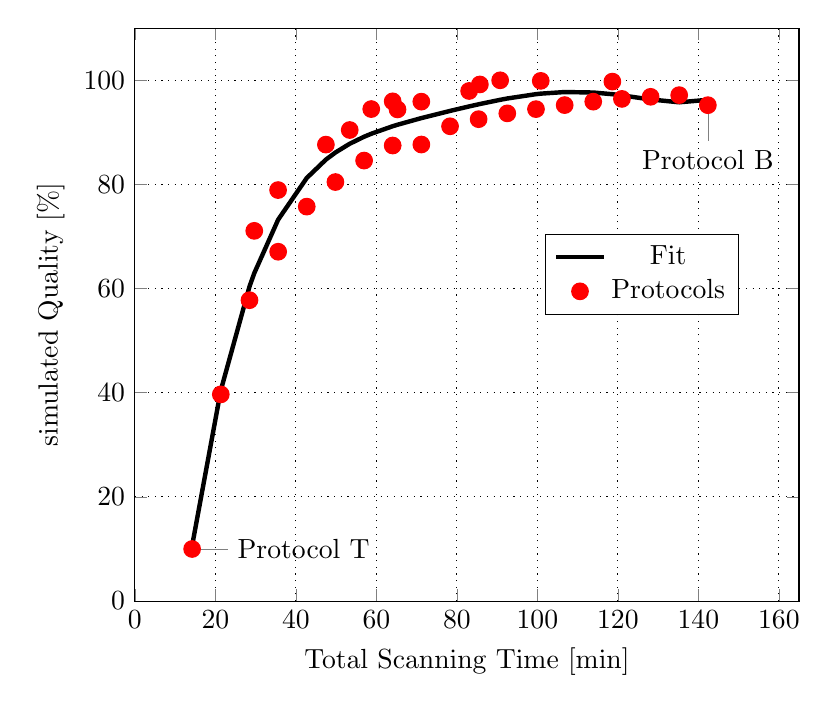
\begin{tikzpicture}[scale = 1]
	
\pgfplotsset{every axis grid/.style={style=dotted}}
\pgfplotsset{every axis legend/.append style={
	at={(.618,.5)},
	anchor=south west}}
%\tikzstyle{every pin}=[fill=white,draw=black,font=\footnotesize]	
\begin{axis}[%
name=main plot,%
axis on top,%
%width=110mm,%
%height=150mm,%
scale only axis,%
xtick={0,20,40,60,80,100,120,140,160},%
ytick={0,20,40,60,80,100},%
xlabel={Total Scanning Time [min]},%
ylabel={simulated Quality [\%]},%
%title={Quality plotted vs. sorted Total Number of Projections},%
xmin=0, xmax=165,%
ymin=0, ymax=110,%
xmajorgrids,%
ymajorgrids%
]
% Line plot
\addplot [%
%color=blue,%
solid,%
ultra thick%line width=1pt%
] coordinates{
 (14.225,10.6329) (21.35,40.4553) (28.475,60.387) (29.66668,62.9627) (35.58332,73.2208) (35.6,73.2445) (42.7,81.239) (47.4584,84.771) (49.8252,86.1369) (53.3752,87.8158) (56.95,89.1628) (58.7252,89.7344) (64.05,91.1798) (64.05,91.1798) (65.25,91.4648) (71.1668,92.7408) (71.1748,92.7425) (78.3,94.1216) (83.0416,94.9832) (85.4,95.3925) (85.7084,95.4449) (90.75,96.2518) (92.5252,96.5086) (99.65,97.3378) (100.8332,97.4378) (106.7752,97.7453) (113.8752,97.6536) (118.6252,97.3285) (121,97.1035) (128.1252,96.3198) (135.2248,95.7766) (142.35,96.253)
};
\addlegendentry{Fit}
% Line plot
\addplot [%
color=red,%
mark size=3.0pt,%
only marks,%
mark=*,%
mark options={solid}%
] coordinates{
 (14.225,10) (21.35,39.688) (28.475,57.7757) (29.66668,71.0901) (35.58332,78.9237) (35.6,67.0809) (42.7,75.7439) (47.4584,87.6519) (49.8252,80.4642) (53.3752,90.4546) (56.95,84.587) (58.7252,94.4763) (64.05,95.9593) (64.05,87.4792) (65.25,94.4094) (71.1668,95.8992) (71.1748,87.669) (78.3,91.1688) (83.0416,97.9498) (85.4,92.5337) (85.7084,99.2014) (90.75,100) (92.5252,93.6496) (99.65,94.4659) (100.8332,99.8906) (106.7752,95.2383) (113.8752,95.899) (118.6252,99.7503) (121,96.4271) (128.1252,96.8306) (135.2248,97.1499) (142.35,95.2221)
};
\addlegendentry{Protocols}

\node[coordinate,pin=right:Protocol T]
at (axis cs:14.225,10) {};
\node[coordinate,pin=below:Protocol B]
at (axis cs:142.35,95.2221) {};
\end{axis}
  
\end{tikzpicture}

%\tikzstyle{every pin}=[fill=white,
%draw=black,
%font=\footnotesize]
%\begin{tikzpicture}
%\begin{axis}[
%xlabel={\textsc{Dof}},
%ylabel={$L_2$ Error}]
%\addplot coordinates {
%(11, 10)
%(71, 100)
%(351, 350)
%};
%\node[coordinate,pin=above:Bad!]
%at (axis cs:10,10) {};
%\node[coordinate,pin=left:Good!]
%at (axis cs:71,250) {};
%\end{axis}
%\end{tikzpicture}

%\end{document}
	\caption{Quality-Plot of 32 calculated protocols. The red dots mark the properties of the protocols, the plot is a fifth-order polynomial fit. 19 of these protocols have been scanned and are discussed in section~\ref{sec: Results I}.}
	\label{af}
\end{figure}

\section{Results II}
Results of the steps mentioned in section~\ref{sec:materials and methods} are shown in figure~\ref{fig:wide field scan results}. Figure~\ref{fig:subscans} shows exemplary projection images from overlapping subscans prior to correction and normalization. Figure~\ref{fig:merge-proj} shows a merged projection image prior to reconstruction and figure~\ref{fig:merge-rec} shows the end-result of such a wide field scan, a reconstructed slice of the whole sample with a FOV of \SI{5.734}{\milli\meter} which is  approximately three times the size of what can be achieved with one single scan.

\begin{figure*}[p]
	\renewcommand{\imsize}{.16\linewidth}
	\pgfmathsetlength{\imagewidth}{\imsize} % desired display width of image
	\pgfmathsetlength{\imagescale}{\imagewidth/512} % pixel width of image
	\centering
		\subfloat[Uncorrected projection images from subscans s$_1$--s$_3$, each with a size of 1024$\times$1024 pixels at a resolution of \SI{1.4}{\micro\meter\per pixel}, covering a FOV of approximately \SI{0.7}{\milli\meter}. The scans overlap each other by approximately 100 pixels. 4676 projections have been acquired for the subscans s$_1$ and s$_3$, 1169 projections have been acquired for subscan s$_2$, all over a rotation of \SI{180}{\degree}.]{%
			\label{fig:s1}%
			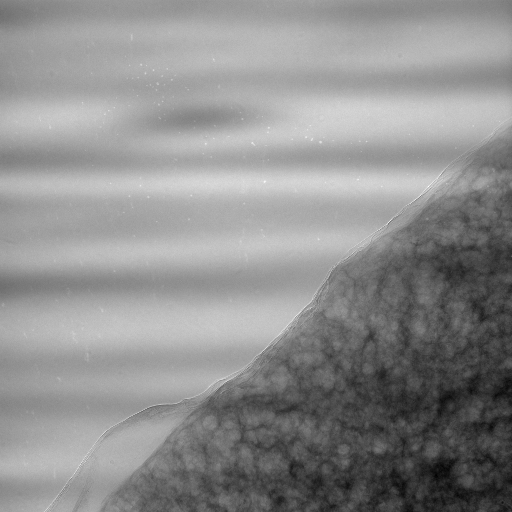
\includegraphics[width=\imsize]{img/merge/R108C10B-s1}%
			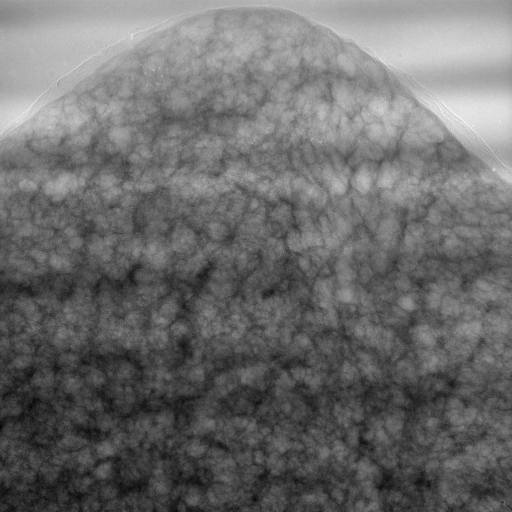
\includegraphics[width=\imsize]{img/merge/R108C10B-s2}%
			\begin{tikzpicture}[x=\imagescale,y=-\imagescale]
				% place image (integer coordinates refer to pixel centers):
				\node[anchor=north west,inner sep=0pt,outer sep=0pt] at (0,0)
					{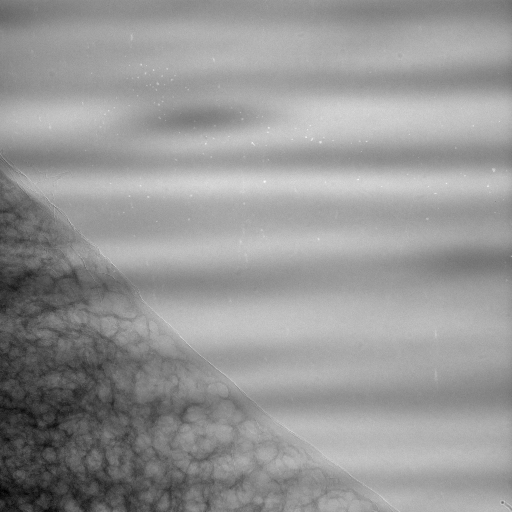
\includegraphics[width=\imagewidth]{img/merge/R108C10B-s3}};
				\draw[|-|,color=white] (256-64,450) -- (512-64,450) node[midway,above] {\SI{700}{\micro\meter}};
			\end{tikzpicture}
			\label{fig:subscans}
			}
		\renewcommand{\imsize}{.48\linewidth}
		\pgfmathsetlength{\imagewidth}{\imsize} % desired displayed width of image
		\pgfmathsetlength{\imagescale}{\imagewidth/1498} % pixel width of image
		\subfloat[Merged and corrected image from the three subscans shown in subfigure~\subref{fig:subscans}. The merged projections have a size of 2994$\times$1024 pixels at a resolution of \SI{1.4}{\micro\meter\per pixel}. The Subscans s$_1$--s$_3$ overlap each other by approximately 150 pixels, thus the width of the merged projection is smaller than three times the width of the subscans. The projections of the subscans above have been merged into 4676 projections images like the one shown here and were then reconstructed into a tomographic dataset using a filtered backprojection reconstruction algorithm.]{%
			\begin{tikzpicture}[x=\imagescale,y=-\imagescale]
				\node[anchor=north west,inner sep=0pt,outer sep=0pt] at (0,0)
					{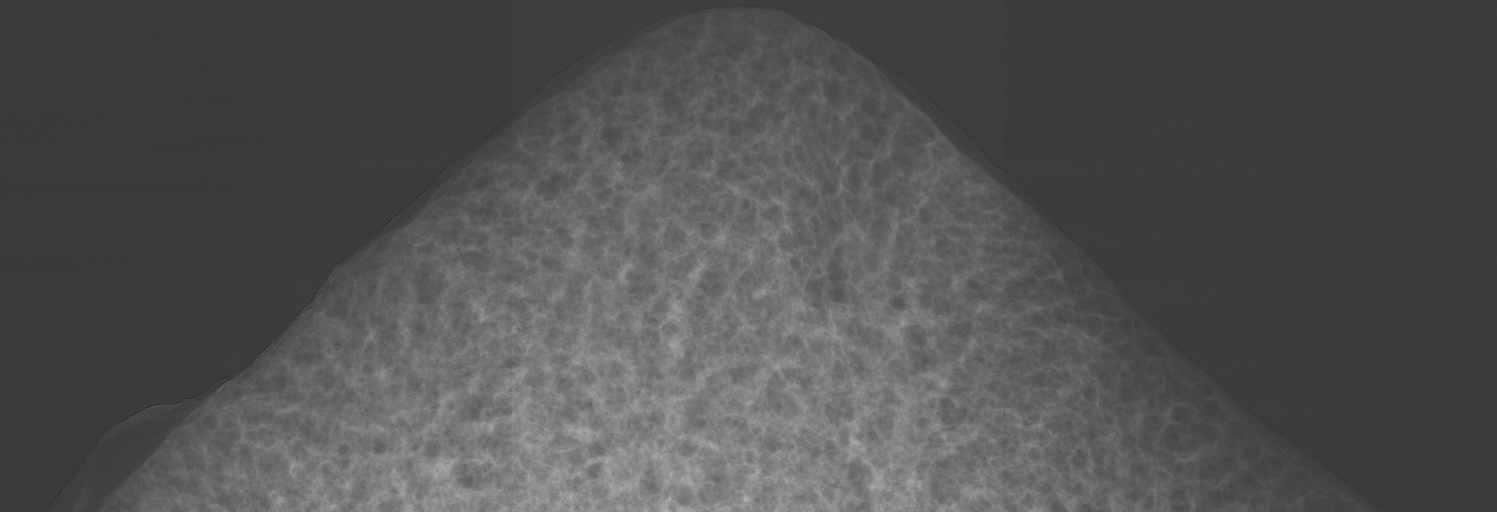
\includegraphics[width=\imagewidth]{img/merge/R108C10B-merge}};
				\draw[|-|,color=white] (1242-64,450) -- (1498-64,450) node[midway,above] {\SI{700}{\micro\meter}};
			\end{tikzpicture}
			\label{fig:merge-proj}
			}
		\renewcommand{\imsize}{\linewidth}
		\pgfmathsetlength{\imagewidth}{\imsize} % desired displayed width of image
		\pgfmathsetlength{\imagescale}{\imagewidth/1365} % pixel width of image (image has been resized from 2994*1123, so that scalebar is at the same height without calculating too much...)
		\subfloat[Cropped part of one slice of the tomographic dataset reconstructed from the merged projections, where one is shown in subfigure~\subref{fig:merge-proj}. The halo directly around the lung tissue arises from the paraffin where the sample is embedded in. The bright circular shape inscribed in the square arises from the filtered backprojection, the chosen reconstruction method. The size of the cropped image is 2994$\times$1123 pixels. The small inset on the upper left corner shows an overview over the full slice with a size of 2994$\times$2994 pixels.]{%
			\begin{tikzpicture}[x=\imagescale,y=-\imagescale]
				% place image (integer coordinates refer to pixel centers):
				\node[anchor=north west,inner sep=0pt,outer sep=0pt] at (0,0)
					{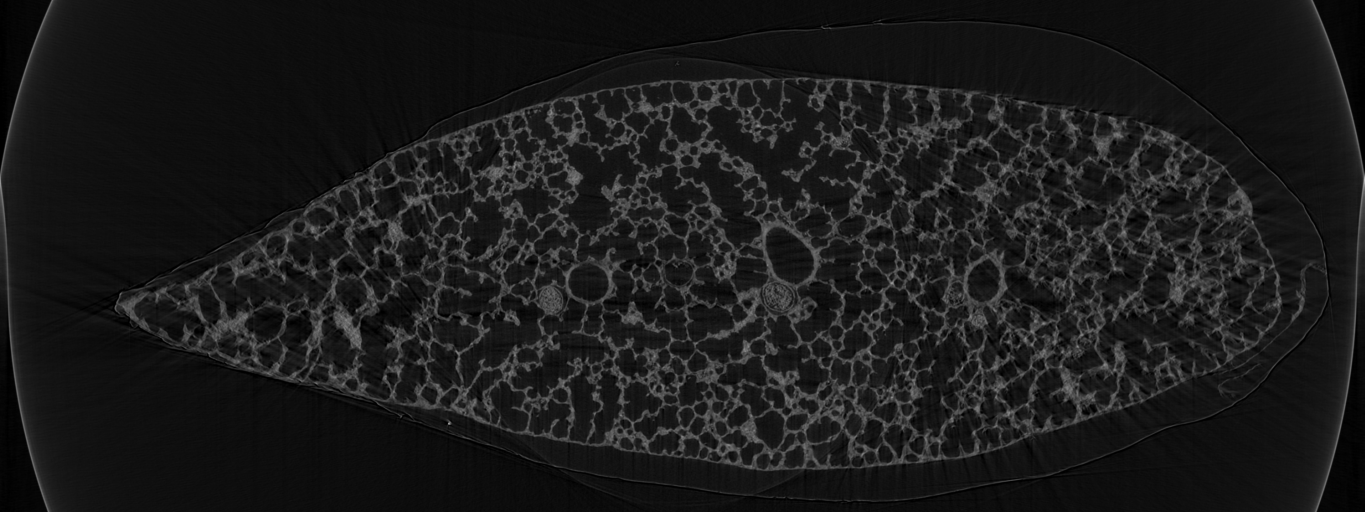
\includegraphics[width=\imagewidth]{img/merge/R108C10B-merge1016-crop}};
				\newcommand{\size}{.2\imagewidth}
				\node[anchor=north west,inner sep=0pt,outer sep=0pt] at (0,0)
					{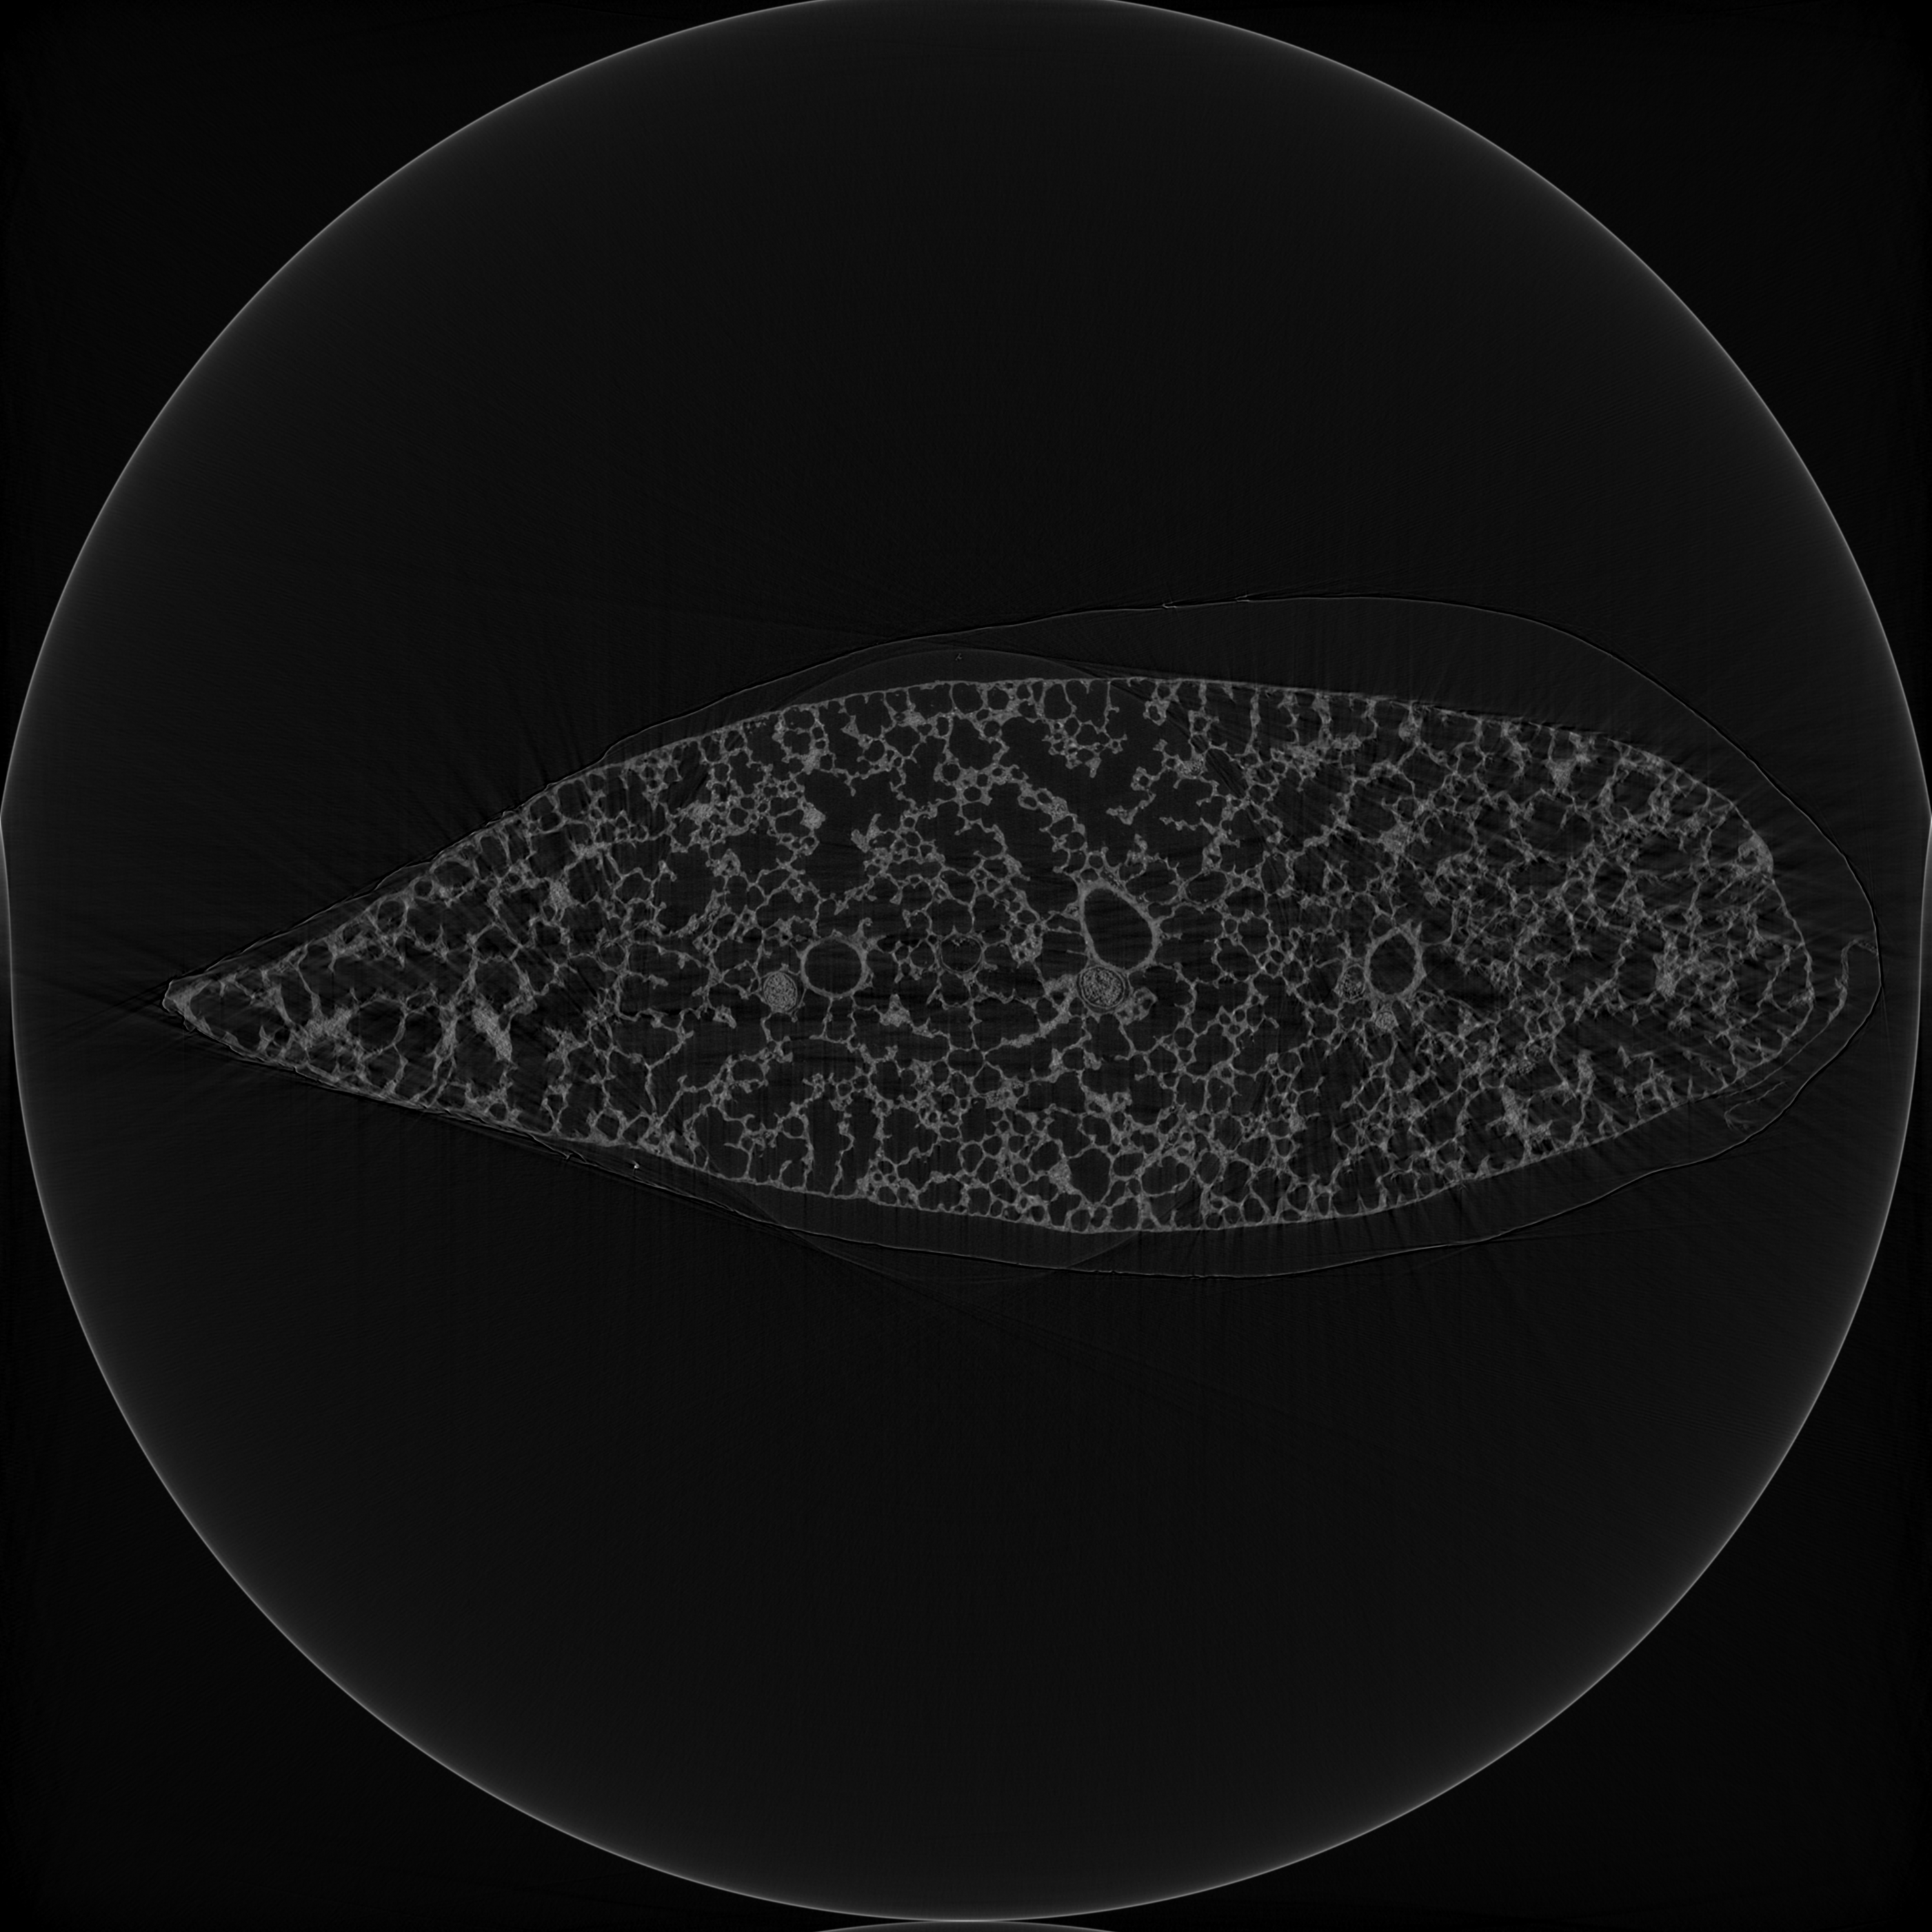
\includegraphics[width=\size]{img/merge/R108C10B-merge1016}};
					\draw[white] (\size,0) -- (\size,-\size) -- (0,-\size);
				\draw[|-|,color=white] (1109-64,450) -- (1365-64,450) node[midway,above] {\SI{700}{\micro\meter}};
			\end{tikzpicture}
			\label{fig:merge-rec}
			}
	\caption{Different stages of a wide field scan of a rat lung sample obtained from a Sprague-Dawley rat 10 days after birth, showing the distal-medial edge of the right lower lung lobe. The sample has been scanned at a beam energy of \SI{12.6}{\kilo\electronvolt}.}
	\label{fig:wide field scan results}	
\end{figure*}

\begin{itemize}
	\item Problems with insufficient sampling for outer subscans?
	\item Stitching takes long time (incorporation into \verb+prj2sin+ and \verb+sin2rec+ @ beamline?)
\end{itemize}

\begin{itemize}
	\item MATLAB \& Python-Script prior to imaging
	\begin{itemize}
		\item integration with robot $>$ potentially eliminating any user intervention with sample placement.
	\end{itemize}
	\item automatically scanning all subscans, no user intervention.
	\item MATLAB-stitching after imaging
	\item RecoManager
	\begin{itemize}
		\item \verb+gridrec+-Problem solved?
	\end{itemize}
\end{itemize}

\begin{figure}[p]
	\renewcommand{\imsize}{\linewidth}
	\pgfmathsetlength{\imagewidth}{\imsize} 		 % desired displayed width of image
	\pgfmathsetlength{\imagescale}{\imagewidth/1589} % 1589*728 = width of imagefile used below
	\newcommand{\startx}{982} %= 1589*.618
	\newcommand{\starty}{655} %= 728*.9
	\centering
	\subfloat[]{
		\begin{tikzpicture}[x=\imagescale,y=-\imagescale]
 			\node[anchor=north west,inner sep=0pt,outer sep=0pt] at (0,0)
 			{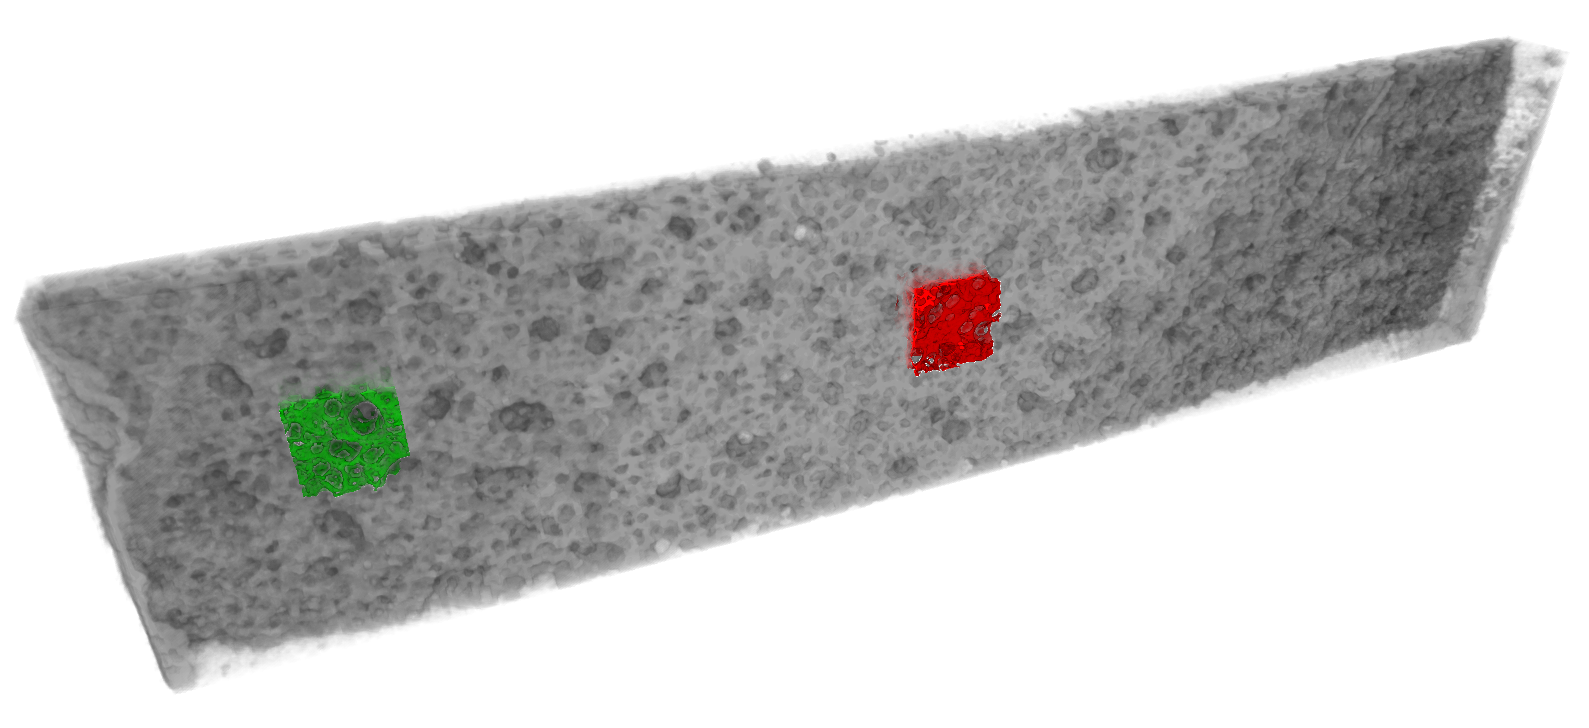
\includegraphics[width=\imagewidth]{img/sophie/full}};
 			\draw[|-|](\startx-808,\starty) -- (\startx+500,\starty) node[midway,above] {\SI{3.3978}{\milli\meter}}; % 4854px * 0.7 um/px = 3.3978 mm
	 	\end{tikzpicture}
	 	\label{subfig:LungSlab}
		}
	\renewcommand{\imsize}{.25\linewidth}
	\pgfmathsetlength{\imagewidth}{\imsize} % desired displayed width of image
	\pgfmathsetlength{\imagescale}{\imagewidth/902} % 1543*928 = width of imagefile used below
	\renewcommand{\startx}{557} %= 902*.618
	\renewcommand{\starty}{802} %= 891*.9
	\subfloat[]{%
		\begin{tikzpicture}[x=\imagescale,y=-\imagescale]
			\node[anchor=north west,inner sep=0pt,outer sep=0pt] at (0,0)
 			{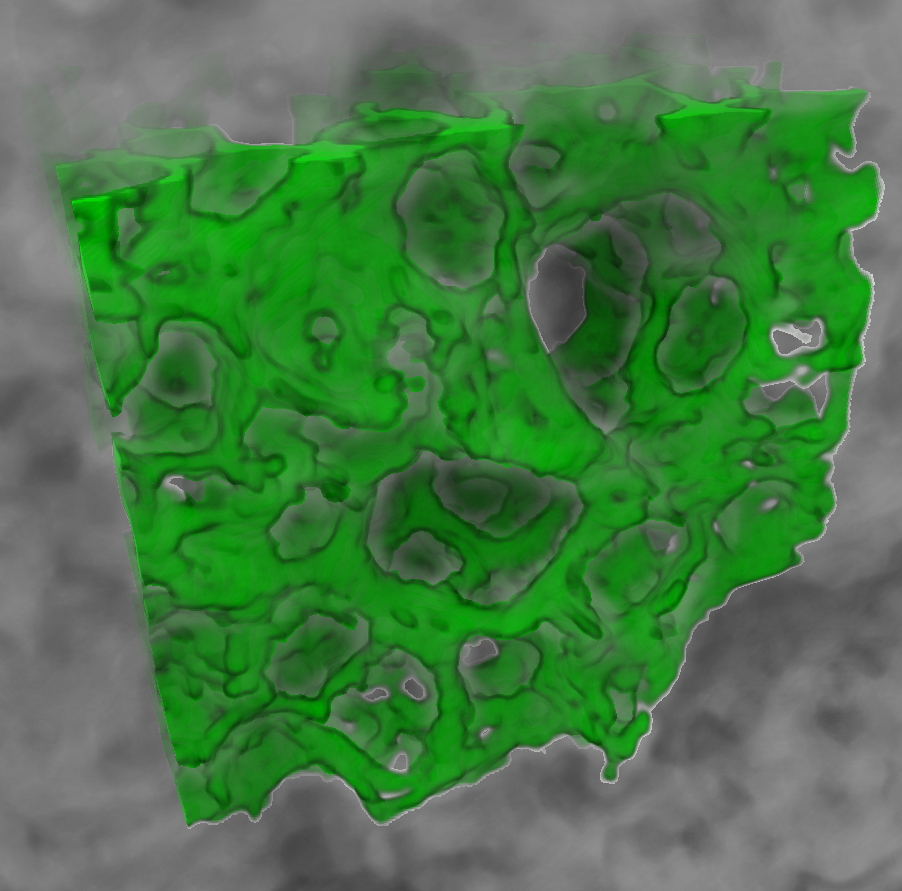
\includegraphics[width=\imagewidth]{img/sophie/crop-green-background}};
 			\draw[|-|] (\startx+0,\starty) -- (\startx+200,\starty) node[midway,above] {\SI{179.2}{\micro\meter}}; % cube with 256 px = 179.2 um
	 	\end{tikzpicture}%
	  	\label{subfig:LungSlabDetailsGreenBG}%
		}
	\subfloat[]{%
		\begin{tikzpicture}[x=\imagescale,y=-\imagescale]
			\node[anchor=north west,inner sep=0pt,outer sep=0pt] at (0,0)
 			{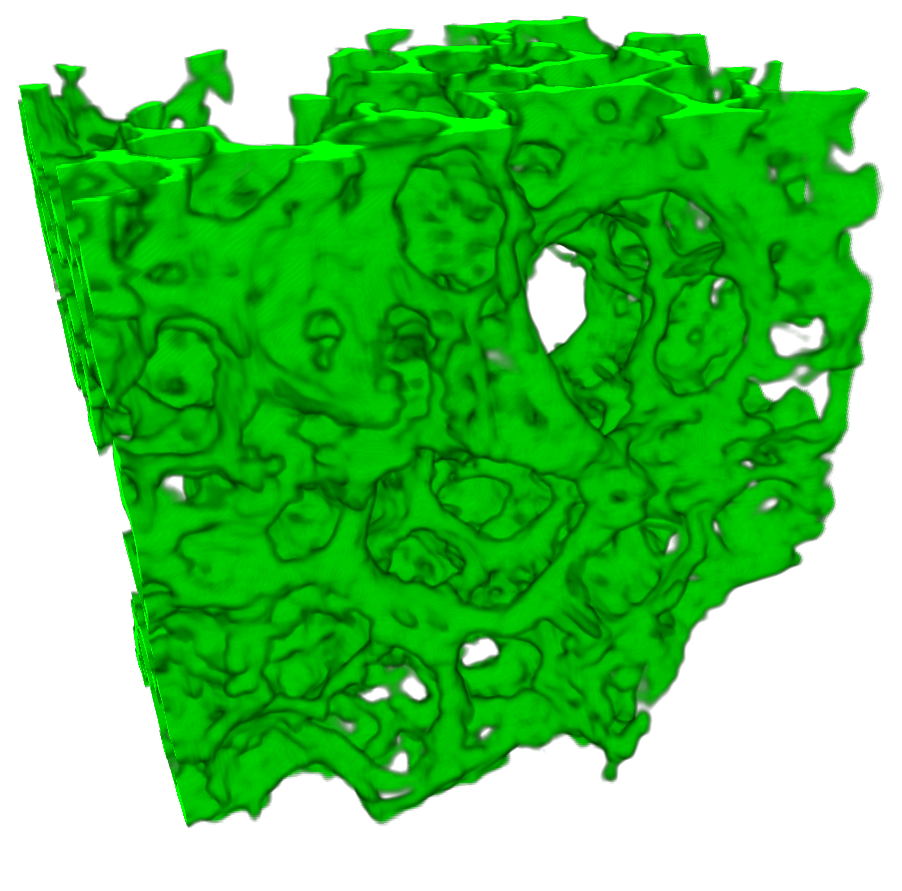
\includegraphics[width=\imagewidth]{img/sophie/crop-green}};
 			\draw[|-|] (\startx+0,\starty) -- (\startx+200,\starty) node[midway,above] {\SI{179.2}{\micro\meter}}; % cube with 256 px = 179.2 um
	 	\end{tikzpicture}%
	 	\label{subfig:LungSlabDetailsGreen}%
		}%
	\subfloat[]{%
		\begin{tikzpicture}[x=\imagescale,y=-\imagescale]
			\node[anchor=north west,inner sep=0pt,outer sep=0pt] at (0,0)
 			{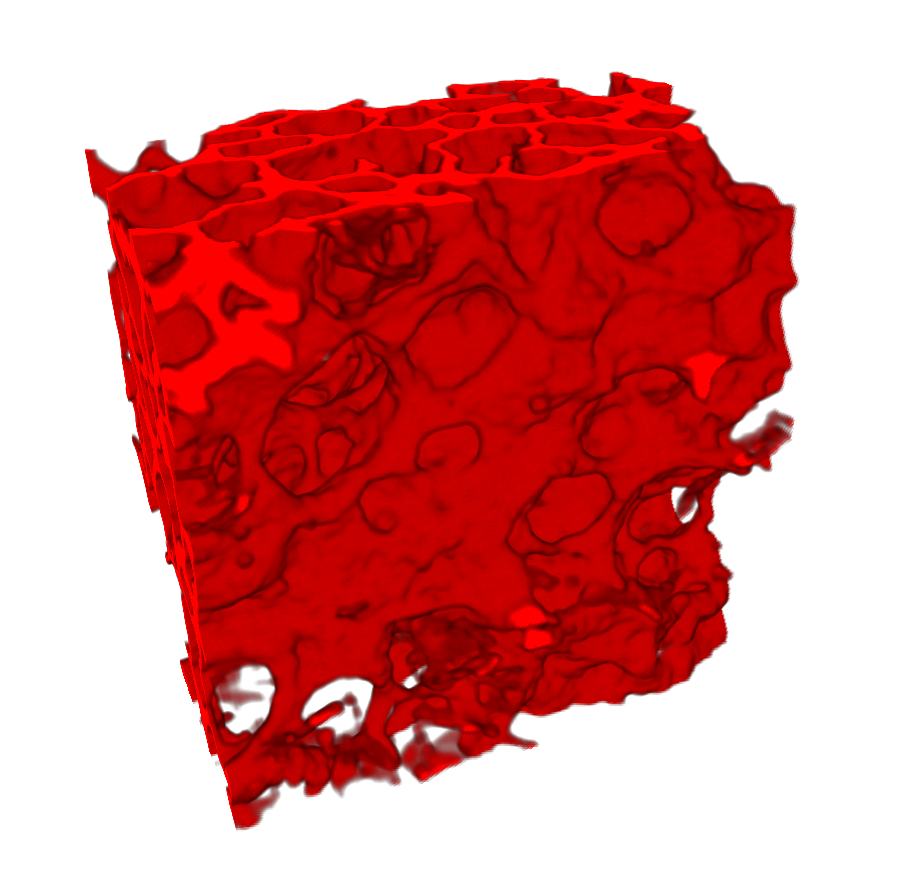
\includegraphics[width=\imagewidth]{img/sophie/crop-red}};
 			\draw[|-|] (\startx+0,\starty) -- (\startx+200,\starty) node[midway,above] {\SI{179.2}{\micro\meter}}; % cube with 256 px = 179.2 um
	 	\end{tikzpicture}%
	  	\label{subfig:LungSlabDetailsRed}%
		}
	\subfloat[]{%
		\begin{tikzpicture}[x=\imagescale,y=-\imagescale]
			\node[anchor=north west,inner sep=0pt,outer sep=0pt] at (0,0)
 			{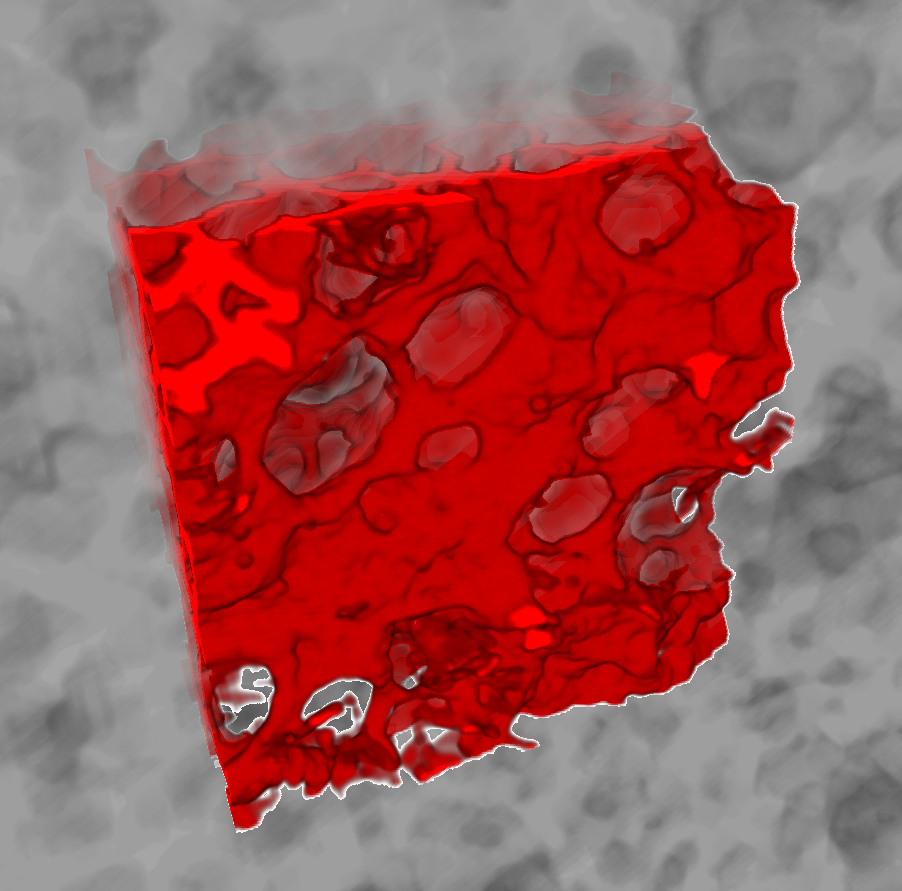
\includegraphics[width=\imagewidth]{img/sophie/crop-red-background}};
 			\draw[|-|] (\startx+0,\starty) -- (\startx+200,\starty) node[midway,above] {\SI{179.2}{\micro\meter}}; % cube with 256 px = 179.2 um
	 	\end{tikzpicture}%
	 	\label{subfig:LungSlabDetailsRedBG}%
		}
	\label{fig:LungSlabSophie}%
	\caption{Visualization of lung tissue slab: %
		\subref{subfig:LungSlab}: Three dimensional volume rendering of slab of lung tissue with a size of 554$\times$4854$\times$1024 pixels at a voxel size of \SI{0.7}{\micro\meter} per pixel. Both inset cubes have a side length of 256 pixels and were automatically segmented using a region growing algorithm. 
 		\subref{subfig:LungSlabDetailsGreenBG}: Closeup of inset cube at an outer position in the sample, including the background tissue. % 
 		\subref{subfig:LungSlabDetailsGreen}: Closeup of inset cube at an outer position in the sample. Albeit we have been able to automatically segment the lung tissue, segmentation artifacts are visible. Single alveoli can be distinguished. %
 		\subref{subfig:LungSlabDetailsRed}: Closeup of inset cube at a central position in the sample. Single alveoly are clearly visible. %
 		\subref{subfig:LungSlabDetailsRedBG}: Closeup of inset cube at a central position in the sample, including the background tissue. %
		The scale bars are only approximate, since it is a three-dimensional view.  The top scale bar is valid for the longest length of the gray lung structure, the bottom scale bar is valid for the width of the red cube.%
	}
	\todo[inline]{adapt the scalebars to the final size of the images}
\end{figure}